% -*- root: warwickthesis.tex -*-

\section{Introduction}
\label{sec:introduction-cell}

% The question we try to answer in this Chapter is, "what if the initial population is heterogeneous?".

In STAMM an important assumption is that the initial cell population is homogeneous. For the applications we discussed in previous Chapters, this assumption is likely to be fulfilled  as experiments are designed to ensure initial homogeneity. In the case of the oncogenic transformation, a cell line is used as the initial cell population. In the case of stem cell reprogramming the technique outlined by \cite{Hanna:2009ix} tries to ensure initial homogeneity  by using a secondary MEF cells.

Recently it has been shown that even seemingly homogeneous cell populations exist in inherent mixtures, be it at an epigenetic level \citep{Heng:2009em,Gerlinger:2012wu}. Without knowing the distribution of the initial population it is not possible to apply STAMM to determine individual states as the solution to the master equation would be incomplete (see eqn.   \ref{eq:masterMat} and eqn.   \ref{eq:state-occ}). In this Chapter, we outline a model that answers the question: What effect does the initial cell population have on cell fate?


\begin{figure}[h]
  \centering
  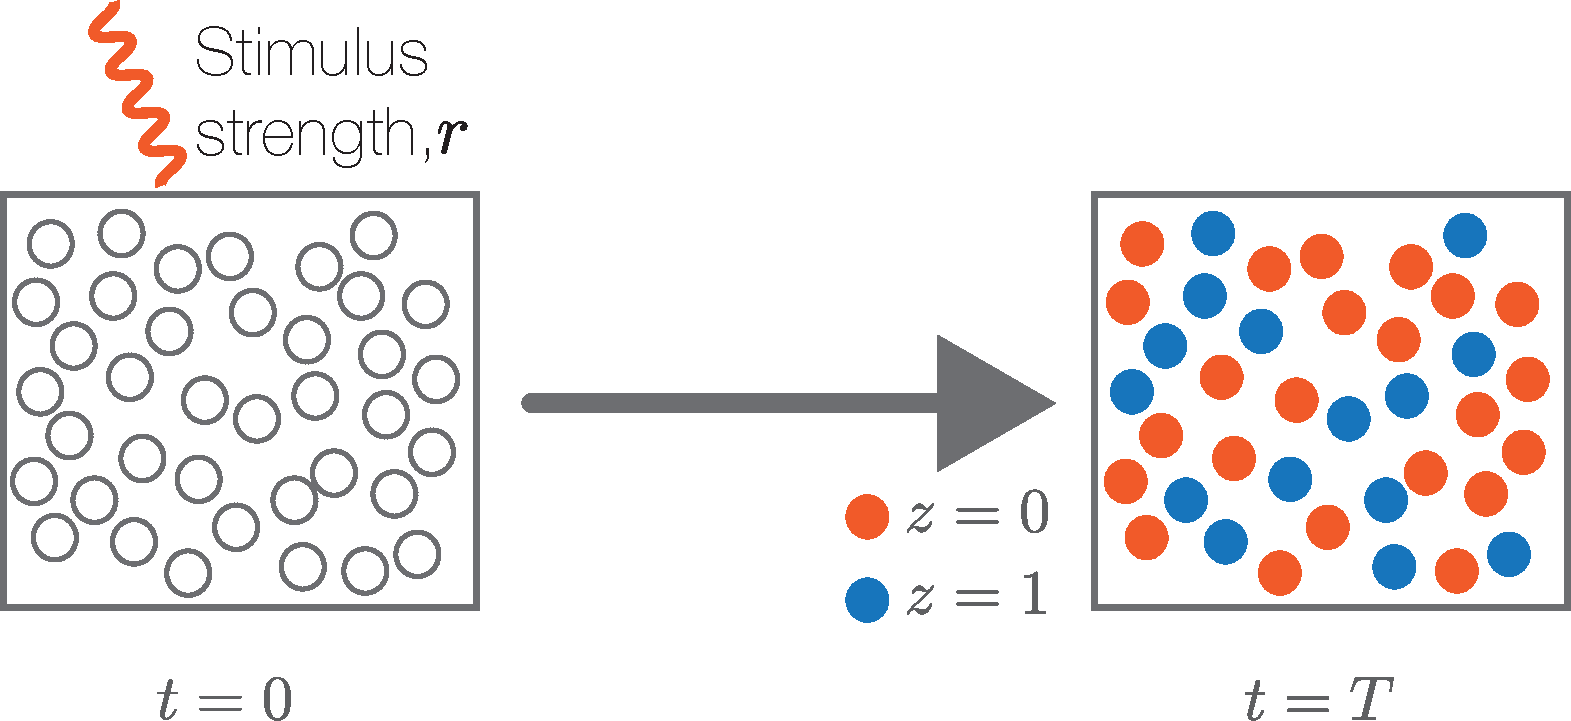
\includegraphics[width=0.7\textwidth]{pics/cell-cycle-model.pdf}
  \caption{Schematic of model. A heterogeneous cell population (the source of heterogeneity is unknown) is at rest at $t=0$, at which point it is perturbed by an external stimulus of strength $r$; evoking a transformation such that two distinct populations form at a later time $t=T$. At $t=T$ it is possible to count the number of cells in different states. }
  \label{fig:cell-cycle-model}
\end{figure}

An example of such a biological system is one with an initial heterogeneous cell population made up of two types of cells, with an indistinguishable phenotype. At time $t=0$ the cells receive a stimulus leading to a transformation such that at $t=T$ it is possible to distinguish cells in their final cell fate. It is possible to count the fraction of cells that reach each of those final cell fates. The question of interest here is whether the strength of the stimulus has an effect on the fraction of cells in each cell fate and how cell fate is related to the expression level of individual genes. A schematic of such a system is shown in Figure \ref{fig:cell-cycle-model}. As the two cell populations have a different stimulus response and we are interested in the influence of gene expression on the response, individual genes influential in determining cell fate are deemed important if their expression level is significantly different between cell populations at $t=0$.

The idea for this model arose from discussions with the Medema lab at the NKI and was originally motivated by their interest in cell cycle biology. The possible experimental application for this model was not ready in time for this thesis therefore all simulation parameters are merely chosen to ensure a full range of stimulus response starting from very few cells responding to a weak stimulus, after which the stimulus is increased until all cells respond and share the same cell fate at $t=T$. The chosen parameter might not bear resemblance to their counterparts in a real biological system; but this model serves as a proof of concept and as long as the basic principles hold, it can be applied to a real system.

We start this Chapter in Section \ref{sec:model-descr} with the basic concepts, introducing variables and deriving  behaviour of such a system followed by the derivation of a model that can be used to estimate parameters given possible measurements on the system. After that we set up a simulation procedure in Section \ref{sec:simulation}. Finally in Section \ref{sec:results-cc} we present results using simulated data, first with only one gene and then with four genes.

\section{Formal system description}
\label{sec:model-descr}

\subsection{Setup}
\label{sec:concepts}

% To formalise model description we derive it

Suppose at time $t$ cell $i$ (out of $N$ cells) occupies state $X_{t}^{(i)}$; where state here broadly refers to any aspect of the cell's physical configuration. This can include protein profile, transcription, or its chromatin state. Denote ultimate cell fate at $t=T$ for cell $i$ by $Z_i$. Cell fate $Z_i$ is determined experimentally by enumerating cells in distinguishable states at $t=T$. In the simplest case cells can have two distinct final states; we label the two states $Z_i = 0$ and $Z_i = 1$. We expect the process that determines cell fate to have a stochastic component such that two physically identical cell at $t=0$ can end up in distinct final states. Hence we assume the probability that cell $i$ is in state $Z_i = 1$ at $t=T$ depends on two things:

\begin{itemize}
\item The physical state of cell $i$ at $t=0$, $X_{0}^{(i)} $.
\item The dose of the stimulus, $r$.
\end{itemize}

We assume that the fraction of cells that reach the arrested state changes with the strength of the stimulus. The fraction of cells that reach cell fate $Z_i = 1$ is dose dependant and the measured fraction at $t=T$ is denoted by $\pi(r)$.

\subsection{Model}
\label{sec:model-cell}

First, we will set up the model in a general sense to give a birds-eye view of the system we are attempting to study. After that, we will derive from this picture the specific model, which is applicable to data that can be realistically observed. In this Chapter, focused on concepts, it is important to first outline overall ideas to ensure the actual model can be fully explained.

We start with formalising the variables. Set the expression of gene $j$ in cell $i$ measured at time $t $ under stimulus strength $r$ to $X_{jt}^{(i)}(r)$. In the first instance we are only going to consider one gene therefore we initially drop the subscript $j$ to make the derivation clearer. When we are referring to measurements at $t=0$ they are independent of the stimulus, therefore we write $X_0^{(i)}(r) = X_0^{(i)}$. The probability of observing a gene expression conditional on the strength of the stimulus can be written as a combination of distinct populations present:

\begin{align}
  p(X_{t}^{(i)} | r) &= p(X_{t}^{(i)}, Z_i =1 | r) + p(X_{t}^{(i)}, Z_i =0 | r)\\
  &= p(X_{t}^{(i)}| Z_i =1,  r) \, p(Z_i =1 | r) + p(X_{t}^{(i)}| Z_i =0,  r) \, p(Z_i =0 | r).
  \label{eq:cond-prob-obs}
\end{align}
Now the expected value for the expression, conditional on the strength of the stimulus, can be calculated using the results of eqn. (\ref{eq:cond-prob-obs}) as:

\begin{align}
  \mathbb{E} [X_t^{(i)} | r] &= \int X_t^{(i)} \; p(X_t^{(i)}| r) dX_t^{(i)} \\
  \begin{split}
    &= p(Z_i = 1| r)\; \int X_t^{(i)} \; p(X_t^{(i)}|Z_i = 1, r) dX_t^{(i)} + \label{eq:exp-cond-cc} \\
    & \; + p(Z_i = 0| r)\; \int X_t^{(i)} \; p(X_t^{(i)}|Z_i = 0, r) dX_t^{(i)}.
  \end{split}
\end{align}
Introducing the new variable $\pi(r) = p(Z_i = 1 | r)$, and for a two state system naturally  $1 - \pi(r) = p(Z_i = 0 | r)$ we rewrite eqn. (\ref{eq:exp-cond-cc})

\begin{equation}
  \mathbb{E} [X_t^{(i)} | r] = \pi(r)\; \mathbb{E} [X_t^{(i)} | Z_i =1, r] + \left( 1 - \pi(r) \right)\; \mathbb{E} [X_t^{(i)} | Z_i =0, r].
\end{equation}
To simplify the notation and write a general equation for a system of this type we rewrite the expected value of the expression level for cells in state $Z_i = 1$ and $Z_i = 0$ as $\alpha(r) = \mathbb{E} [X_t^{(i)} | Z_i =1, r]$ and  $\beta(r) =  \mathbb{E} [X_t^{(i)} | Z_i = 0, r]$ respectively and write:

\begin{equation}
  \label{eq:general-cc}
  \mathbb{E} [X_t^{(i)} | r] = \pi(r) \, \alpha(r) + \left( 1 - \pi(r) \right) \, \beta(r).
\end{equation}
In the biological system described above gene expression is measured at $t=0$ and is independent of the applied stimulus since it is only applied at the initial time point. Therefore we define the expected value of measured expression reintroducing gene $j$,  $\mathbb{E}[X_{t=0}^{(i)} | r] = X_0 $, as:

\begin{equation}
  \label{eq:init-cc}
  X_{0j} = \pi(r) \, \alpha_j(r) + \left( 1 - \pi(r) \right) \, \beta_j(r).
\end{equation}

The system is now fully described, potential measurements that can be made here are the average expression levels of genes at $t=0$, $X_{0j}$ and the fraction of cells in state $Z = 1$ at time $t=T$. On account of the lack of information about the variables $\alpha(r)$ and $\beta(r)$ or their distribution, estimation using eqn. (\ref{eq:init-cc}) is not feasible. Therefore, below we formulate a procedure to estimate parameters that would allow us to determine genes that significantly influence the transition between states under a stimulus.

\subsubsection{Estimation}
\label{sec:estimation-cc}

We start by defining the fraction of cells in state $Z_i = 1$ at $t = T$, note that the derivation in the following few lines is equivalent for cells where $Z_i =0 $. We will perform the detailed calculation for only one case. Here it is also easier to use $\mathbf{X_0}$ as a vector notation for $X_{0j}$

\begin{align}
  \label{eq:3}
  \pi(r) \equiv p(Z_i=1| r) &= \int p(Z_i=1 | \mathbf{X_0},r) p(\mathbf{X_0}|r) d\mathbf{X_0} \\
  &= \int f(\mathbf{X_0};r, \theta) p(\mathbf{X_0}|r) d\mathbf{X_0} \label{eq:simp-cc},
% \end{align}
\intertext{where in eqn. (\ref{eq:simp-cc}) we have replaced $p(Z_i=1 | \mathbf{X_0},r)$ by a general parametric function of the gene expression dependent on the stimulus and a set of parameters $\theta$, $f(\mathbf{X_0};r, \theta) $. Since $p(\mathbf{X_0}|r)$ is the probability distribution of gene expression at time $t=0$ over all cells a good approximation to this process is the exponential distribution; the parameter $\lambda_j$ of the exponential distribution can be set to the measured gene expression for gene $j$ at $t=0$ and will be different for every gene. Therefore we can rewrite eqn. (\ref{eq:simp-cc}) as:}
% \begin{align}
p(Z_i=1| r)  &= \mathbb{E}[f(\mathbf{X}_{0};r,\theta)]_{Exp(\lambda_j)}.
\label{eq:integral}
\end{align}
The expression in eqn. (\ref{eq:integral}) is general and allows for an expression depending on the problem being investigated. Obtaining a closed form solution of the expectation value is only possible for special cases. For the biological system we present below there is no closed form solution. Hence, we propose a numerical approximation using a Monte Carlo integration. We can therefore write:

\begin{equation}
  \label{eq:monte-carlo-cc}
  \pi(r) \approx \frac{1}{N} \sum_{n = 1}^N f(\mathbf{X}_0^{(n)}; r, \theta),
\end{equation}
where each component of the vector $\mathbf{X}_0^{(n)}$ is sampled from the exponential distribution. In each case, it has to be considered if a simple application is sufficient, or if there is need for a more involved algorithm. To identify the optimal set of parameters in the estimation we perform a grid search over all parameters and compare the residual sum of squares (RSS) between observation and estimation using eqn. (\ref{eq:monte-carlo-cc}).

\subsubsection{Application to the cell cycle}
\label{sec:application-cc}

A biological system where the model described above could be applied to is cell cycle arrest due to radiation. The system is quite simple a population of cells is exposed to varying levels of radiation starting at $t=0$. The expression level of these cells is measured using RNA-Seq. At a later time $t=2h$ cells reach two possible states: (i) arrest leading to cell death, or (ii) the cell still has the ability to enter cell cycle and replicate. The fraction of cells in either state can be counted at $t=2h$. In this application, increasing the dose of radiation of course decreases the number of cells that can re-enter the cell cycle. It is of interest to distinguish discriminatory factors for both cells that determine ultimate fate of a cell.

In this application we have a few simple relationships that our choice of $f(\mathbf{X}_0^{(n)}; r, \theta)$ has to obey. Below a certain radiation threshold the effect of radiation will be negligible, and above a certain radiation threshold almost all cells will arrest. Under such constraints, the best choice is a sigmoid of the form:

\begin{equation}
  \label{eq:sigmoid-cc}
  f(\mathbf{X}_0^{(n)}; r, \theta) = \frac{1}{1 + \exp ( -r\, \mathbf{a}^T \mathbf{X_0^{(n)}} + b)},
\end{equation}
where $\mathbf{a}$ and $b$ are parameters of the sigmoid to be determined from estimation. A large negative or positive value in $\mathbf{a}$ for a gene means it has a larger influence on transformation.

\section{Simulation}
\label{sec:simulation}

The simulation setup we choose for this model is based on a single-cell level approach which we employ in Section \ref{sec:sim-study} obtaining very useful results. The first step is to simulate gene expression for each gene and a fixed number of cells; this is sampled from an exponential distribution for each gene $Exp(\lambda_j)$. Then the probability of being in state $Z_i = 1$  is determined using eqn. (\ref{eq:sigmoid-cc}) based on expression levels of all genes involved and fixed radiation value and parameters  $\mathbf{a}$ and $b$. Drawing a value uniformly at random in the range $[0, 1]$ determines for each cell if it is in the arrest state. Using this final state vector we can determine $\pi(r)$. Measurements for such a system will be limited so we repeat these simulation steps for only $9$ values of $r$. Since in a real experiment measurements of fraction of cells will be noisy, we add Gaussian noise to the fraction of cells observed with zero mean $\mathcal{N}(0, \sigma)$, .

\begin{figure}[!t]
  \centering
  \includegraphics[width=1\textwidth]{pics/cell-cycle-sim1.pdf}
  \caption{Single cell simulation for one gene. Plots show the states of cells at different expression levels after exposure to radiation $r$ for $t=2h$. Each figure represents a different dose of radiation $r$. The $y$-axis shows expression level and the x-axis is just an index over 2000 cells which are used in the simulation. State $Z_i = 0$ is the normal state of the cell and state $Z_i =1$ is when cells enter the arrest state. }
  \label{fig:rad-single-gene}
\end{figure}

\section{Results}
\label{sec:results-cc}

\subsection{Single gene simulation}
\label{sec:single-gene-simul}

Initially we perform the simulation and estimation with only a single gene. This is to determine whether or not it is possible to estimate parameters for the simplest possible case. We perform simulations for $1000$ cells for one gene with $Exp(\lambda_j = 5)$ at $r = \lbrace 0, 0.1, 0.5, 1, 2, 3, 5, 6, 10 \rbrace$. The sigmoid parameters are chosen as $a = 2$ and $b = 5$. To visualise the single cell simulation behaviour Figure \ref{fig:rad-single-gene} shows the states occupied at $t = 2h$ by $1000$ cells at different radiation doses. The y-axis in the plot represents gene expression transformed for convenience to $\arcsinh(X_0)$. Once we have obtained values for $\pi(r)$ from this setup we add two levels of Gaussian noise $\sigma = \lbrace 0.025, 0.05, 0.1 \rbrace$. Since the measured quantity is in the range $[0, 1]$ this is a reasonable level of noise, ranging from $2.5 \%$ to $10 \%$ of the simulated trajectory. Finally we choose a grid for $b$ over the interval $[0, 10]$ and $a$ over the interval $[0, 4]$ and find the minimal RSS. The results from these estimations are summarised in Table \ref{tab:fit-cc-single}. We see that for $\sigma = 0.025$ the estimates are very close to the true values used in simulation. At higher noise, the estimates become progressively worse, but the parameter order is still preserved.

\begin{table}[!t]
    \centering
\begin{tabular}{r||c|rrr}
  \hline \hline
   & true value & $\sigma = 0.025$ & $\sigma = 0.05$ & $\sigma = 0.1$ \\
  \hline
  $a$ & 2 & 1.655 & 1.124 & 0.828 \\
  $b$ & 5 & 4.483 & 3.448 & 2.759 \\
   \hline
 \end{tabular}
 \caption{Estimation of $a$ and $b$ parameters from simulated data. Data is obtained by adding Gaussian noise to the simulated trajectory with different $\sigma$ values. }
 \label{tab:fit-cc-single}
\end{table}

\subsection{Simulation with multiple genes}
\label{sec:simul-with-mult}
\begin{figure}
  \centering
  \subfigure[$\sigma = 0.05$]{
    \includegraphics[width=0.45\textwidth]{pics/cc-4gn-1.pdf}
    \label{fig:4gn-5}
  }
  \subfigure[$\sigma = 0.1$]{
    \includegraphics[width=0.45\textwidth]{pics/cc-4gn-2.pdf}
    \label{fig:4gn-10}
  }
  \caption{Simulation study. Ten simulations carried out with four genes.  The expression for genes in each cell are sampled from an exponential distribution with the mean chosen uniformly between $[0, 20]$, stimuli used at $r =\lbrace 0, 0.1, 0.5, 1, 2, 3, 5, 6, 10 \rbrace$. Parameters for the simulation is chosen as $b=5$ and $a=[1, 5, 10, 0.2]$ for the simulation. \subref{fig:4gn-5} is the simulations with Gaussian noise added at $\sigma = 0.05$. The estimated parameters are ranked in the correct order. \subref{fig:4gn-10} is the simulation performed where additive Gaussian noise has $\sigma = 0.1$. Here parameter estimation is worse, but not unexpected since the noise added is at $10\%$ of the observed data values.}
  \label{fig:cc-4gn}
\end{figure}

Just performing simulation using a single gene only serves to show the simulation pipeline and as a first test to determine if the model will work. If we wish to determine how well the proposed model will serve in a realistic application it is necessary to expand the simulation to include multiple genes, otherwise the model is not useful. To this end we implement a simulation with $4$ genes. Just like above we perform a simulation with $1000$ genes measured at $r =\lbrace 0, 0.1, 0.5, 1, 2, 3, 5, 6, 10 \rbrace$. We choose the parameters as follows $b=5$ and $a=[1, 5, 10, 0.2]$ and the mean gene expression for each gene is drawn uniformly between $[0, 20]$. To estimate parameters we apply a grid over all parameters calculating the integral eqn. (\ref{eq:monte-carlo-cc}) with the Monte carlo approximation and find the parameter set that minimises RSS. This is of course a very inefficient  method,  and with increase in parameters, the grid search quickly becomes unfeasible. A more sophisticated implementation of parameter selection is necessary for a realistic application.  We repeat this simulation $10$ times with independently drawn over expression and we repeat this for two different standard deviations of noise added to the fraction of transformed cells $0.05$ and $0.1$. Figure \ref{fig:cc-4gn} shows the results for both noise levels and we can see that for lower noise the estimation works well and parameters are estimated in the right order. For larger noise, this is already difficult and some parameters are estimated well and some are not.



\section{Discussion}
\label{sec:discussion-cc}

We derived the model starting from general biological principles including a description of the system. We introduced one possible application for this model in a radiated cell population either stopping cells in cell cycle or only temporarily halting it. In such an experiment, we wanted to find the importance of genes for the transformation.  In this model, there is one parameter that determines the importance of genes. The higher the value for a gene the more important that gene is in transformation. We showed in simulation that we can obtain parameters even when we add large amounts of noise to the simulated data in a single gene scenario. With limited observations made on the system (the initial gene expression and proportions of cells reaching a specific cell fate for different stimuli) we are interested in finding out if the level of expression of a gene influences cell fate. It will not be possible to estimate exact parameter values. We show that it is possible to obtain ranks of genes using this model.

For a real application, further work is needed. Only with real data comparison is it possible to determine if the choices made for parameters during simulation are reasonable and if simulated state fractions are realistic. Further work is also needed to implement a more useful parameter search instead of the crude one implemented at the moment. Once it can be compared to data, it will also be possible to refine the model if needed.


%%% Local Variables:
%%% TeX-master: "warwickthesis"
%%% End:
